\documentclass{article}

\PassOptionsToPackage{numbers, compress}{natbib}
% Camera ready: \usepackage[final]{nips_2017}
\usepackage{nips_2017}

\usepackage[utf8]{inputenc} % allow utf-8 input
\usepackage[T1]{fontenc}    % use 8-bit T1 fonts
\usepackage{hyperref}       % hyperlinks
\usepackage{url}            % simple URL typesetting
\usepackage{booktabs}       % professional-quality tables
\usepackage{amsfonts}       % blackboard math symbols
\usepackage{nicefrac}       % compact symbols for 1/2, etc.
\usepackage{microtype}      % microtypography
\usepackage{graphicx}
\usepackage{algorithm}% http://ctan.org/pkg/algorithms
\usepackage{algpseudocode}% http://ctan.org/pkg/algorithmicx
\usepackage{booktabs}
\usepackage{subfigure}

\usepackage{amsmath}
\usepackage{amssymb}
\usepackage{amsfonts}
%\usepackage{enumerate}
%\usepackage{bbm}
%\usepackage{caption}

\newcommand{\pa}[1]{ \left({#1}\right) }

\def \N {\mathbb{N}}
\def \Nbr {\mathcal{N}}
\def \Q {\mathbb{Q}}
\def \F {\mathbb{F}}
\def \then {\implies &}
\def \oif {\Longleftrightarrow &\,}
\def \given {\text{Given }&}
\def \assume {\text{Assume }&}
\def \thfr {\therefore &\enskip}
\def \bij {\leftrightarrow}
\def \inj {\rightarrowtail}
\def \sur {\twoheadedrightarrow}
\def \Z {\mathbb{Z}}
\def \R {\mathbb{R}}
\def \C {\mathbb{C}}
\def \T {\mathbb{T}}
\def \iff {\Longleftrightarrow}
\def \kron {\boldsymbol\delta}
%\def \indicator {\mathbbm{1}}

\def\tbr{{\textbf{r}}}
\def\Ts{\textbf{s}}
\def\Ta{\textbf{a}}
\def\Tm{\textbf{m}}
\def\Tb{\textbf{b}}
\def\Tc{\textbf{c}}
\def\Td{\textbf{d}}
\def\Te{\textbf{e}}
\def\Tv{\textbf{v}}
\def\Tx{\textbf{x}}
\def\TX{\textbf{X}}
\def\TU{\textbf{U}}
\def\Tu{\textbf{u}}
\def\Ty{\textbf{y}}
\def\Tk{\textbf{k}}
\def\Tt{\textbf{t}}
\def\Tz{\textbf{z}}
\def\quotient{\mathclose{}/\mathopen{}}
\def\Tf{\textbf{f}}
\def\Th{\textbf{h}}
\def\Tg{\textbf{g}}
\def\sumn{\sum_{n=0}^\infty}
\def\limn{\lim_{n\rightarrow\infty}}
\def\prodn{\prod_{n=0}^\infty}

\def\bsz{\textbf{0}}
\def\bs1{\textbf{1}}
\def\bsa{{\boldsymbol\alpha}}
\def\bse{{\boldsymbol\eta}}
\def \bss{ {\boldsymbol\sigma}}

\DeclareMathOperator{\conv}{conv}
\DeclareMathOperator\cat{cat}
\DeclareMathOperator\adj{adj}
\DeclareMathOperator\Pois{Pois}
\DeclareMathOperator\Id{Id}
\DeclareMathOperator\mathProb{\mathbb{P}}
\def\P{\mathProb} % need to overwrite stupid paragraph symbol
\DeclareMathOperator\mathExp{\mathbb{E}}
\def \E {\mathExp}


\newcommand{\stc}[1]{\widetilde{#1}}   
\newcommand{\set}[2]{ \left\{ #1 \,\middle|\, #2 \right\} }
\newcommand{\idx}[3]{ \left\{ #1 \right\}_{ #2 }^{ #3 } }
\newcommand{\shift}[1]{&\quad & \text{#1}\\}
\newcommand{\lem}[1]{\text{\textbf{L.\ref{#1}}}}
\newcommand{\card}[1]{\left\vert{#1}\right\vert}
\newcommand{\colv}[1]{\begin{pmatrix} #1 \end{pmatrix}}
\newcommand{\mat}[1]{\begin{pmatrix} #1 \end{pmatrix}}
\newcommand{\detmat}[1]{\begin{vmatrix} #1 \end{vmatrix}}
\newcommand{\spanb}[1]{\text{span}\{ #1 \}}
\newcommand{\abs}[1]{\left|#1\right|}
\newcommand{\opcat}[1]{#1^{\text{op}}}
\newcommand{\Inner}[1]{\left\langle #1 \right\rangle}
\newcommand{\Innercpy}[1]{\Inner{ #1, #1 }}
\newcommand{\norm}[1]{\left\| #1 \right\|}% use instead of $\|x\|$

\def\eqd{\mathrel{\overset{\Delta}{=}}}

\DeclareMathOperator{\diag}{diag}
\DeclareMathOperator{\vcdim}{VC-dim}
\DeclareMathOperator*{\Err}{\text{err}}
\DeclareMathOperator*{\ErrE}{\mathbb{E}}
\DeclareMathOperator{\Tr}{tr}
\DeclareMathOperator{\Dim}{dim}
\DeclareMathOperator{\Rank}{rank}
\DeclareMathOperator*{\argmin}{argmin}
\DeclareMathOperator*{\proj}{proj}
\DeclareMathOperator{\Ker}{ker}
\DeclareMathOperator{\Diam}{diam}
\DeclareMathOperator{\Int}{int}
\DeclareMathOperator{\Clo}{clo}
\DeclareMathOperator{\sgn}{sgn}
\DeclareMathOperator{\MyRe}{Re}
\DeclareMathOperator{\MyIm}{Im}
\DeclareMathOperator{\image}{image}
\DeclareMathOperator{\colim}{colim}
\DeclareMathOperator{\Supp}{supp}
\DeclareMathOperator{\Var}{var}
\DeclareMathOperator{\Hom}{hom}
\DeclareMathOperator{\Ob}{ob}
\DeclareMathOperator{\El}{el}
\DeclareMathOperator\power{{\mathcal{P}}}
\DeclareMathOperator{\Nat}{Nat}
\DeclareMathOperator{\cone}{cone}
\DeclareMathOperator{\vectorize}{vec}
\DeclareMathOperator{\matricize}{mat}
\DeclareMathOperator{\cov}{cov}
\DeclareMathOperator{\Unif}{Unif}
\DeclareMathOperator{\blockdiag}{blockdiag}
\DeclareMathOperator{\mvm}{MVM}

% probability stuff
\def \sa {{$\sigma$-algebra}}
\def\OR{{\overline{\R}}}
\def\OX{{\overline{X}}}

\def\mcU{{\mathcal{U}}}
\def \mcX {\mathcal{X}}
\def \mcS {\mathcal{S}}
\def \mcY {\mathcal{Y}}
\def \mcL {\mathcal{L}}
\def \mcD {\mathcal{D}}
\def \mcC {\mathcal{C}}
\def \mcA {\mathcal{A}}
\def \mcK {\mathcal{K}}
\def \mcM {\mathcal{M}}
\def\mcG{{\mathcal{G}}}
\def\mcH{{\mathcal{H}}}
\def\mcF{{\mathcal{F}}}
\def\mcB{{\mathcal{B}}}
\def\mcE{{\mathcal{E}}}
\def\mcI{{\mathcal{I}}}
\def\mcQ{{\mathcal{Q}}}
\def\mcM{{\mathcal{M}}}
\def\mcC{{\mathcal{C}}}
\def\mcT{{\mathcal{T}}}
\def\mcO{{\mathcal{O}}}
\def\mcJ{{\mathcal{J}}}

\def\bsa{{\boldsymbol\alpha}}
\def\bsr{{\textbf{r}}}
\def\bse{{\boldsymbol\epsilon}}
\def\bsk{{\boldsymbol\kappa}}
\def\bsm{{\boldsymbol\mu}}
\def\bsl{{\boldsymbol\lambda}}
\def\bsph{{\boldsymbol\phi}}
\def\bsth{{\boldsymbol\theta}}

\def\abovestrut#1{\rule[0in]{0in}{#1}\ignorespaces}
\def\belowstrut#1{\rule[-#1]{0in}{#1}\ignorespaces}
\def\abovespace{\abovestrut{0.20in}}
\def\belowspace{\belowstrut{0.10in}}


\title{Large Linear Multi-output Gaussian Process Learning for Time Series}

\author{
  Vladimir Feinberg, Li-Fang Cheng, {Barbara Engelhardt}, {Kai Li}\\
  Department of Computer Science\\
  Princeton University\\
  Princeton, NJ 08544 \\
  \texttt{\{vyf,lifangc,bee,li\}@princeton.edu} \\
}

\begin{document}

\maketitle

\begin{abstract}
Gaussian process (GP) models, which put a distribution over arbitrary functions in a continuous domain, can be generalized to the multi-output case; a common way of doing this is to use a linear model of coregionalization (LMC) \cite{alvarez2012kernels}. Such models can learn and exploit correlations across the multiple outputs. For instance, temperature data from disparate regions over time can contribute to a predictive weather model that is more accurate than a single, localized model. While model learning can be performed efficiently for single-output GPs \cite{msgp}, such methods assume stationarity, a luxury unavailable in the multi-output case. We propose Large Linear GP (LLGP), which recovers stationarity thanks to LMC's structure, enabling optimization of GP hyperparameters for multi-dimensional outputs and one-dimensional inputs. Our approach learns hyperparameters at an asymptotically faster rate than the current state of the art. When applied to real time series data, we find this theoretical improvement is realized with LLGP being generally an order of magnitude faster while improving or maintaining predictive accuracy. Finally, we discuss extensions of our approach to multidimensional inputs.
\end{abstract}

% NOTES
% 8 pages of content
% \citet for inline citations
% footnotes after punctuation
% no vertical rules in tables
% \subsubsection*{Acknowledgments} only in final paper

\section{Introduction}\label{introduction}

Gaussian processes (GPs) are a popular nonlinear regression method that innately capture function smoothness across inputs as defined by their covariance function \cite{williams1996gaussian}. GPs seamlessly extend to multi-output learning, picking up on latent cross-output processes, where in multi-output learning the objective is to build a probabilistic regression model over vector-valued observations.

Multiple-output GPs frequently appear in time-series contexts, such as the problem of imputing missing temperature readings for sensors in different locations and reconstructing missing foreign exchange rates and commodity prices given rates and prices for other goods over time \cite{osborne2008towards, alvarez2010efficient}. Efficient model learning would enable researchers to quickly explore large spaces of model configurations to find an appropriate one for their task.

Exact GP inference is infeasible in this scenario since it requires maintaining pairwise covariance between all inputs in a large matrix and performing inversions with that matrix \cite{williams1996gaussian}. As the number of hyperparameters grows, so do the number of matrix operations (Tab.~\ref{asymp}). For this reason, an accurate approximate approach has been an important goal of machine learning research.

\subsection{Contributions}

Our approach makes the following contributions to approximate inference in multi-output GPs, scoped to time series input. First, we identify a block-Toeplitz structure induced by the linear model of coregionalization (LMC) kernel on a grid. Next, we adapt a previously identified kernel structure based on Semiparametric Latent Factor Models (SLFM) \cite{seeger2005semiparametric}. Both of these structures coordinate for fast matrix-vector multiplication $K\Tz$ with the covariance matrix $K$ for any vector $\Tz$.

When inputs do not lie on a uniform grid (for time series, the length of time between observations differs), we demonstrate how to leverage structured kernel interpolation (SKI) in the multi-output setting, where SKI, which requires stationary kernels, does not naturally apply \cite{kiss-gp}. Because LMC kernels exhibit the previously-identified block-Toeplitz structure, they harmonize with SKI.

For low-dimensional inputs, the above contributions offers an asymptotic and practical runtime improvement in hyperparameter learning while also expanding feasible kernel typs to arbitrary differntiable LMC kernels, with improvement taken to be relative to existing multi-GP methods (Tab.~\ref{asymp}) \cite{nguyen2014collaborative}.

Our paper is organized as follows. In Sec.~\ref{sec:background} we give a background on single-output and multi-output GPs, as well as some history in structured linear algebra in GPs. Sec.~\ref{sec:related-work} details both related work that was built upon in LLGP and existing methods for multi-output GPs. Sec.~\ref{sec:matrix-free} describes our method, including a matrix-free heuristic stopping criterion. Then, in Sec.~\ref{sec:results} we compare the performance of LLGP to existing methods and offer concluding remarks in Sec.~\ref{conclusion}.


\section{Background}
\label{sec:background}

\subsection{General Gaussian processes}

First, we give an overview of the theoretical foundation for GPs. A GP is a set of random variables (RVs) $\{f_\Tx\}_\Tx$ indexed by $\Tx\in\mcX$, with the property that for any finite collection $X=\idx{\Tx_i}{i=1}{n}$ of $\mcX$, the RVs are jointly Gaussian \cite{williams1996gaussian}. With zero mean wlog and a prescribed covariance $K:\mcX^2\rightarrow\R$, $\Tf_X\sim N\pa{\bsz, K_{X, X}}$, where $(\Tf_X)_i=f_{\Tx_i}$ and $(K_{X,X})_{ij}=K(\Tx_i,\Tx_j)$. Given observations $\Ty\in\R^n$ of $\Tf_X$, inference at a single point $*\in\mcX$ of an $\R$-valued RV $y_*$ is performed by the marginalization $y_*|\Tf_X$ \cite{williams1996gaussian}.
Predictive accuracy is sensitive to a particular parameterization of our kernel, so model estimation is performed by maximizing data log likelihood with respect to parameters $\bsth$ of $K$, $\mcL(\bsth)=\log p(\Tf_{X}|X,\bsth)$. As such, the heart of GP learning lies in optimization of $\mcL$. Gradient-based optimization methods then require the gradient with respect to every parameter $\theta_j$ of $\bsth$:
\begin{align}
\partial_{\theta_j}\mcL = \frac{1}{2}\bsa^\top\partial_{\theta_j}K_{|\bsth}\bsa -\frac{1}{2}\Tr\pa{K_{|\bsth}^{-1}\partial_{\theta_j}K_{|\bsth}};\;\; \bsa=K_{|\bsth}^{-1}\Ty.\label{llgradient}
\end{align}

\subsection{Multi-output linear GPs}

We build multi-output GP models as instances of general GPs, where a multi-output GP model identifies correlations between outputs through a shared input space \cite{alvarez2012kernels}. Here, for $D$ outputs, we write our indexing set as $\mcX'=[D]\times \mcX$: an input is in a point from a shared domain coupled with an output tag. Then, if we make observations at $X_d\subset\mcX$ for output $d\in[D]$, we can set:
\begin{align*}
\TX=\set{(d, x)}{d\in[D],x\in X_d}\subset{\mcX'};\;\; n=\card{\TX}.
\end{align*}

An LMC kernel $K$ is of the form 
\begin{align}
K([i,\Tx_i],[j,\Tx_j])=\sum_{q=1}^Qb_{ij}^{(q)}k_q(\norm{\Tx_i-\Tx_j})+\epsilon_i1_{i=j},\label{lmcpointwise}
\end{align} 
where $k_q:\R\rightarrow\R$ is a stationary kernel on $\mcX$. Typically, the positive semi-definite (PSD) matrices $B_q\in\R^{D\times D}$ formed by $b_{ij}^{(q)}$ are parameterized as $A_qA_q^\top+\bsk_q I_D$, with $A_q\in\R^{D\times R_q},\bsk_q\in\R_+^D$ and $R_q$ a preset rank. Importantly, even though each $k_q$ is stationary, $K$ is only stationary on $\mcX'$ if $B_q$ is Toeplitz. Settings of $B_q$ that arise in practice, where we wish to capture covariance across outputs as an arbitrary $D^2$-dimensional latent process, prevent stationarity in $K$ and therefore prohibit direct application of SKI.

The LMC kernel provides a flexible way of specifying multiple additive contributions to the covariance between to inputs for two different outputs. The contribution of the $q$-th kernel $k_q$ to the covariance between the $i$-th and $j$-th outputs is then specified by the multiplicative factor $b_{ij}^{(q)}$. By choosing $B_q$ to have rank $R_q=D$, so the contribution between those two outputs is learned independently of all other contributions, the entries of $B_q$. By lowering the rank $R_q$, researchers applying the LMC model can specify that the contributions of the kernels for each output pair are determined by lower-rank latent processes, with rank 0 indicating no interaction (i.e., if $A=0$ then we have an independent GP for each output).

\subsection{Structured covariance matrices}

If we can identify structure in the covariance matrices $K$, then we can recover fast in-memory representations and efficient matrix-vector multiplications (MVMs) for $K$.

The Kronecker product $A\otimes B$ of matrices of order $a,b$ is a block matrix of order $ab$ with $ij$-th block $A_{ij}B$. We can represent it by keeping representations of $A$ and $B$ separately, rather than the product. Then, the corresponding MVMs can be computed in time $O(a\mvm(B)+b\mvm(A))$, where $\text{MVM}(\cdot)$ is the runtime of a MVM. For GPs on uniform dimension-$P$ grids, this approximately reduces the runtime and representation costs by a $(1/P)$-th power \cite{gilboa2015scaling}.

Symmetric Toeplitz matrices $T$ are constant along their diagonal and fully determined by their top row $\{T_{1j}\}_j$, yielding an $O(n)$ representation. Such matrices arise naturally when we examine the covariance matrix induced by a stationary kernel $k$ applied to a one-dimensional grid of inputs. Since the difference in adjacent inputs $t_{i+1}-t_{i}$ is the same for all $i$, we have the Toeplitz property that:
\[
T_{(i+1)(j+1)}=k(\abs{t_{i+1} -t_{j+1}})=k(\abs{t_i-t_j})=T_{ij}
\]
Furthermore, we can embed $T$ in the upper-left corner of a circulant matrix $C$ of twice its size, which enables MVMs $C\mat{\Tx & \textbf{0}}^\top=\mat{T\Tx &\textbf{0}}^\top$ in $O(n\log n)$ time. This approach has been used for fast inference in single-output GP time series with uniformly spaced inputs \cite{cunningham2008fast}.

\section{Related work}
\label{sec:related-work}
\subsection{Approximate inference methods}

To cope with the lack of tractable GP inference methods, inducing point approaches create a tractable model to use instead of the classic GP. Such approaches fix or estimate inducing points $\TU$ and claim that the data $f_X$ is conditionally deterministic (deterministic training conditional, or DTC), independent (fully independent training conditional, or FITC), or partially independent (partially independent training conditional, or PITC) given RVs $f_{\TU}$  \cite{quinonero2005unifying}. These approaches are agnostic to kernel stationarity, and their quality can be improved by increasing the number of inducing points at the cost of a longer runtime. Setting the inducing points $\TU=\TX$ recovers the original exact GP. Computationally, these approaches resemble making rank-$m$ approximations to the $n\times n$ covariance matrix.

\citet{nguyen2014collaborative} observed in Collaborative Multi-output Gaussian Processes (COGP) that multi-output GP algorithms can further share an internal representation of the covariance structure among all outputs at once. COGP further uses a variational approximation, the evidence lower bound, to the log likelihood. COGP supports a subset of LMC kernels, namely those that match the SLFM model \cite{seeger2005semiparametric}. In an LMC representation (Eq.~\ref{lmcpointwise}), these models correspond to all $\bsk_q$ set to 0 and $A_q=\textbf{a}_q\in\R^{D\times 1}$. Moreover, SLFM and COGP models add in an independent GP to each output, represented in LMC as additional kernels $\idx{k_d}{d=1}{D}$, where $A_d=0$ and $\bsk_d=\Te_d\in\R^D$.

\subsection{Approaches for stationary kernels}

\subsubsection{Structured Kernel Interpolation (SKI)}\label{ski-section}

SKI abandons the inducing-point approach: instead of using an intrinsically sparse model, SKI approximates the original $K_{X,X}$ directly \cite{kiss-gp}. To do this efficiently, SKI relies on the differentiability of $K$. For $\Tx,\Tz$ within a grid $U$, $\card{U}=m$, and $W_{\Tx,U}\in\R^{1\times m}$ as the cubic interpolation weights~\cite{keys1981cubic}, $\abs{K_{\Tx,\Tz}-W_{\Tx,U}K_{U,\Tz}}=O(m^{-3})$. The simultaneous interpolation $W\triangleq W_{X,U}\in\R^{n\times m}$ then yields the SKI approximation: $K_{X,X}\approx WK_{U,U}W^\top$. $W$ has only $4^dn$ nonzero entries, with $\mcX=\R^d$.

In order to adapt SKI to our context of multiple outputs, we build grid $\TU\subset\mcX'$ out of a common subgrid $U\subset\mcX$ that extends to all outputs with $\TU = [D]\times U$. Since the LMC kernel evaluated between two sets of outputs $K_{X_i,X_j}$ is differentiable, as long as $U$ contains each $\{X_d\}_{d\in[D]}$, the corresponding SKI approximation $K_{\TX,\TX}\approx WK_{\TU,\TU}W^\top$ holds with the same asymptotic convergence cubic in $1/m$.

Massively Scalable Gaussian Processes (MSGP) observes that the kernel $K_{U,U}$ on a grid exhibits Kronecker and Toeplitz matrix structure \cite{msgp}. Drawing on previous work on structured GPs \cite{cunningham2008fast, gilboa2015scaling}, MSGP uses linear conjugate gradient descent as a method for evaluating $K_{|\bsth}^{-1}\Ty$ efficiently for Eq.~\ref{llgradient}. In addition, \cite{wilson2014fast} mentions an efficient eigendecomposition that carries over to the SKI kernel for the remaining $\log\abs{K_{|\bsth}}$ term in Eq.~\ref{llgradient}.

While evaluating $\log\abs{K_{|\bsth}}$ is not feasible in the LMC setting (because the LMC sum breaks Kronecker and Toeplitz structure), the general notion of creating structure with SKI carries over to LLGP.

\section{Large Linear GP} \label{sec:matrix-free}

We propose a linear model of coregionalization (LMC) method based on recent structure-based optimizations for GP estimation instead of variational approaches. Critically, the accuracy of the method need not be reduced by keeping the number of interpolation points $m$ low because its reliance on structure allows better asymptotic performance.
For simplicity, our work focuses on multi-dimensional outputs, one-dimensional inputs, and Gaussian likelihoods.

For a given $\bsth$, we construct an operator $\tilde{K}_{|\bsth}$ which approximates MVMs with the covariance matrix, $K_{|\bsth}\Tz\approx \tilde{K}_{|\bsth}\Tz$. Using only the action of MVM with the covariance operator, we derive $\nabla\mcL(\bsth)$. Critically, we cannot access $\mcL$ itself, only $\nabla\mcL$, so we choose AdaDelta as the high-level optimization routine for $\mcL$ \cite{zeiler2012adadelta}.

\subsection{Gradient construction}

\citet{gibbs1996cient} describe the algorithm for GP model learning in terms of only MVMs with the covariance matrix. In particular, they note that we can solve for $\bsa$ satisfying $K_{|\bsth}\bsa=\Ty$ in Eq.~\ref{llgradient} using linear conjugate gradient descent (LCG). Moreover, they develop a stochastic approximation by introducing RV $\tbr$ with $\cov \tbr=I$:
\begin{align}
  \Tr\pa{K_{|\bsth}^{-1}\partial_{\theta_j}K_{|\bsth}} = \E\left[(K_{|\bsth}^{-1}\tbr)^\top\partial_{\theta_j}K_{|\bsth}\tbr\right]\label{eq:trace}
\end{align}
For this approximation, the number of samples need not be large, and the estimate improves as the size of $K_{|\bsth}$ increases.
As in other work \cite{cutajar2016preconditioning}, we let $\tbr\sim\Unif\{\pm 1\}$ and take a fixed number of $N$ samples from $\tbr$.

We depart from Gibbs and MacKay in two ways, yielding Algorithm~\ref{alg:grad}. First, we do not construct $K_{|\bsth}$, but a low-memory representation $\tilde{K}_{|\bsth}$, described in Sec.~\ref{fast-mvm}. Second, we select \textsc{minres} instead of LCG as the Krylov-subspace inversion method used to compute inverses from MVMs. \textsc{minres} handles numerically semidefinite matrices with more grace \cite{fong2012cg}. This is essential in GP optimization, where the diagonal noise matrix $\bse$, iid for each output, shrinks over the course of learning, making inversion-based methods require additional iterations because of increases in $\kappa_2$, the spectral condition number of $K$ (Fig.~\ref{fx2007-iterations}).

\begin{figure}[!h]
\centering
\includegraphics[width=0.5\columnwidth]{iterations.eps}
\caption{Number of MVMs that \textsc{minres} must perform at each optimization iteration for a GP applied to the dataset in Sec.~\ref{fx2007-results}. The iteration cutoff is the number of training points $n$ in the dataset.
}
\label{fx2007-iterations}
\end{figure}

Every AdaDelta iteration (invoking Algorithm~\ref{alg:grad}) then takes total time $\tilde{O}(\mvm(\tilde{K}_{|\bsth})\sqrt{\kappa_2})$ \cite{raykar2007fast}. This analysis holds as long as the error in the gradients is fixed and we can compute MVMs with the matrix $\partial_{\theta_j}K_{|\bsth}$ for each $j$ at least as fast as $\mvm({\tilde{K}_{|\bsth}})$. Indeed, we assume a differentiable kernel and then recall that applying the linear operator $\partial_{\theta_j}$ will maintain the structure of $K_{|\bsth}$.

\begin{algorithm}[!ht]
  \caption{Compute an approximation of $\nabla L$. Assume \textsc{minres} is the inversion routine. We also assume we have access to linear operators $D_{\theta_j}$, representing matrices $\partial_{\theta_j}\tilde{K}_{|\bsth}$.} \label{alg:grad}
\begin{algorithmic}[1]
  \Procedure{LLGP}{$\tilde{K}_{|\bsth}$, $\Ty$, $N$, $\{D_{\theta_j}\}$}
  \State $R\gets\idx{\tbr_i}{i=1}{N}$, sampling $\tbr\sim\Unif\{\pm 1\}$.
\For{$\Tz$ in $\{\Ty\}\cup R$, in parallel}
\State $K^{-1}\Tz\gets\textsc{minres}(\tilde{K}_{|\bsth},\Tz)$.
\EndFor
\State $g\gets \bsz$
\For{$\theta_j$ in $\bsth$}\Comment{Compute $\partial_{\theta_j}\mcL$}
\State $t\gets \frac{1}{N}\sum_{i=1}^{N}\pa{K^{-1}\tbr_i}\cdot D_{\theta_j}(\tbr_i)$\Comment{$t$ approximates the trace term of Eq.~\ref{eq:trace}}
\State $g_j\gets \frac{1}{2}\pa{K^{-1}\Ty}\cdot \tilde{K}_{|\bsth}\pa{K^{-1}\Ty}-\frac{1}{2}t$\Comment{Eq.~\ref{llgradient}}
\EndFor
\State \Return $g$ 
\EndProcedure
\end{algorithmic}
\end{algorithm}

\subsection{Fast MVMs and parsimonious kernels}\label{fast-mvm}

The bottleneck of Algorithm~\ref{alg:grad} is the iterative MVM operations in $\textsc{minres}$. Since $K_{|\bsth}$ only enters computation as an MVM operator, the amount of memory consumed is dictated by its representation $\tilde{K}_{|\bsth}$, which need not be dense, so long as it can reconstruct multiplication with any vector to arbitrary, fixed precision.

When LMC kernels are evaluated on a grid of points for each output, so $X_d=U$, the simultaneous covariance matrix equation without noise Eq.~\ref{lmcgrid} over $\TU$ holds for Toeplitz matrices $K_q$ formed by the stationary kernels $k_q$ evaluated at pairs of $U\times U$, the shared interpolating points for all outputs:
\begin{align}
  K_{\TU,\TU}=\sum_q(A_qA_q^\top+\diag\bsk_q)\otimes K_q\label{lmcgrid}.
\end{align}

Importantly, the Kronecker structure of Eq.~\ref{lmcgrid} lets us re-use the same grid $K_q$ in a computational sense across the different outputs. Recalling our SKI extension to multiple outputs (Sec.~\ref{ski-section}), we build a corresponding approximation for the differentiable part of our kernel:
\begin{align}
  K_{\TX,\TX}\approx WK_{\TU,\TU}W^\top+\bse.\label{lmcski}
\end{align}
We cannot fold $\bse$ into the interpolated term $K_{\TU,\TU}$ since it does not correspond to a differentiable kernel, so the SKI approximation fails. But this fact does not prevent efficient representation or multiplication since the matrix is diagonal. Then, the MVM operation $K_{\TX,\TX}\Tz$ can be approximated by $WK_{\TU,\TU}W^\top\Tz+\bse\Tz$, where matrix multiplication by the sparse matrices $\bse, W,W^\top$ require $O(n)$ space and time.

We consider different representations of $K_{\TU,\TU}$ from (Eq.~\ref{lmcski}) to reduce the memory and runtime overhead for performing the multiplication $K_{\TU,\TU}\Tz$ in the following sections.

\subsubsection{\textsc{sum}: sum representation}

In \textsc{sum}, we represent $K_{\TU,\TU}$ with a $Q$-length list. At each index $q$, $B_q$ is a dense matrix of order $D$ and $K_q$ is a Toeplitz matrix of order $m$, with only the top row maintained. In turn, multiplication $K_{\TU,\TU}\Tz$ is performed by multiplying each matrix in the list with $\Tz$ and summing the results. As described before, the Kronecker MVM $(B_q\otimes K_q)\Tz$ may be expressed as $D$ fast Toeplitz MVMs with $K_q$ and $m$ dense MVMs with $B_q$. In turn, assuming $D\ll m$, the runtime for each of the $Q$ terms is $O(Dm\log m)$.

\subsubsection{\textsc{bt}: block-Toeplitz representation}

In \textsc{bt}, we notice that $K_{\TU,\TU}$ is a block matrix with blocks $T_{ij}$:
\begin{align*}
\sum_qB_q\otimes K_q =\mat{T_{ij}}_{i,j\in[D]^2},\;\; T_{ij}=\sum_qb_{ij}^{(q)}K_q.
\end{align*}
On a one-dimensional grid $U$, these matrices are Toeplitz since they are linear combinations of Toeplitz matrices. \textsc{bt} requires $D^2$ $m$-sized rows to represent each $T_{ij}$. Then, using usual block matrix multiplication, an MVM $K_{\TU,\TU}\Tz$ takes $O(D^2m\log m)$ time.

On a grid of inputs with $\TX=\TU$, the SKI interpolation vanishes with $W=I$. In this case, using \textsc{bt} alone leads to a faster algorithm---applying the Chan block-Toeplitz preconditioner in a Krylov-subspace based routine has experimentally shown convergence of Krylov-based inversion routines using fewer MVMs \cite{chan1994circulant}.

\subsubsection{\textsc{slfm}: SLFM representation}

For the rank-based \textsc{slfm} representation, let $R\triangleq \nicefrac{\sum_qR_q}{Q}$ be the average added rank, $R\le D$, and re-write the kernel:
\begin{align*}
  K_{\TU,\TU}=\sum_q\sum_{r=1}^{R_q}\textbf{a}_q^{(r)}{\textbf{a}_q^{(r)}}^\top\otimes K_q + \sum_q\diag\bsk_q \otimes K_q.
\end{align*}
Note $\textbf{a}_q^{(r)}{\textbf{a}_q^{(r)}}^\top$ is rank-1. Under some re-indexing $q'\in[RQ]$ which flattens the double sum such that each $q'$ corresponds to a unique $(r, q)$, the term $\sum_q\sum_{r=1}^{R_q}\textbf{a}_q^{(r)}{\textbf{a}_q^{(r)}}^\top\otimes K_q $ may be rewritten as
\begin{align*}
  \sum_{q'}\textbf{a}_{q'}\textbf{a}_{q'}^\top\otimes K_{q'} = \textbf{A}\blockdiag_{q'}\colv{K_{q'}}\textbf{A}^\top;
\end{align*}
where $\textbf{A}=\mat{ \textbf{a}_{q'}}_{q'}\otimes I_m$ with $\mat{ \textbf{a}_{q'}}_{q'}$ a matrix of horizontally stacked column vectors \cite{seeger2005semiparametric}. Next, we rearrange the remaining term $\sum_q\diag\bsk_q \otimes K_q$ as $\blockdiag_d(T_d)$, where $T_d=\sum_q \kappa_{qd}K_q$ is Toeplitz. Thus, the \textsc{slfm} representation writes $K_{\TU,\TU}$ as the sum of two block diagonal matrices of block order $QR$ and $D$, where each block is a Toeplitz order $m$ matrix, so MVMs take $O((QR + D)m\log m)$ time.

Because the runtimes of \textsc{bt} and \textsc{slfm} are complimentary in the sense that one performs better than the other when $D^2>QR$ and vice-versa, an algorithm that uses the aforementioned condition between to decide between which representation to use can minimize runtime (Tab.~\ref{asymp}). We also found that \textsc{sum} is efficient in practice for $Q=1$.

\begin{table}[!h]
  \caption{
   For both LLGP and COGP, $m$ is a configurable parameter which increases up to $n$ to improve accuracy. $Q,R,D,\kappa_2$ are coefficients dependent on the setting of the LMC kernel, which has about $QRD$ hyperparameters (Eq.~\ref{lmcpointwise}). The resulting asymptotic performance is given in the table. COGP is only independent of $R$ because it cannot represent models for $R\neq 1$. We distinguish in the up-front cost and per-hyperparameter cost for computing $\nabla \mcL$ to capture the varying asymptotic behaviors of the gradient algorithms as the number of hyperparemters increases: the total cost would be the up-front cost plus $QRD$ multiplied by the per-hyperparameter cost.
  }
\label{asymp}
\begin{sc}
\begin{center}
\begin{small}
\begin{tabular}{ccc}
  \toprule
  Method & Up-front cost for $\nabla \mcL$ & \begin{tabular}{c}Additional cost for $\partial_{\theta_j}\mcL$\\ per hyperparameter\end{tabular}\\
  \midrule
  Exact & $n^3$ & $n^2 $\\
  COGP & $Qm^3$ & $nm$ \\
  LLGP & $\min(QR, D^2)\sqrt{\kappa_2} (n + m\log m)$ &  $n + m\log m$ \\
  \bottomrule
\end{tabular}
\end{small}
\end{center}
\end{sc}
\end{table}

\subsection{Stopping conditions}\label{stopping}

For a gradient-only stopping heuristic, we maintain the running maximum gradient $\infty$-norm. If gradient norms drop below a preset proportion of the running maximum norm more than a pre-set tolerance number of times, we terminate. For example, when applied to the foreign exchange rate prediction dataset in Sec.~\ref{fx2007-results}, the heuristic eventually notices that we have slowed down increases in $\mcL$ because the gradients occasionally drop below the threshold at that point, while not displacing the solution $\bsth$ significantly since we must be near a local minimum (Fig.~\ref{fx2007-stop}). 

\begin{figure}[!h]
\centering
{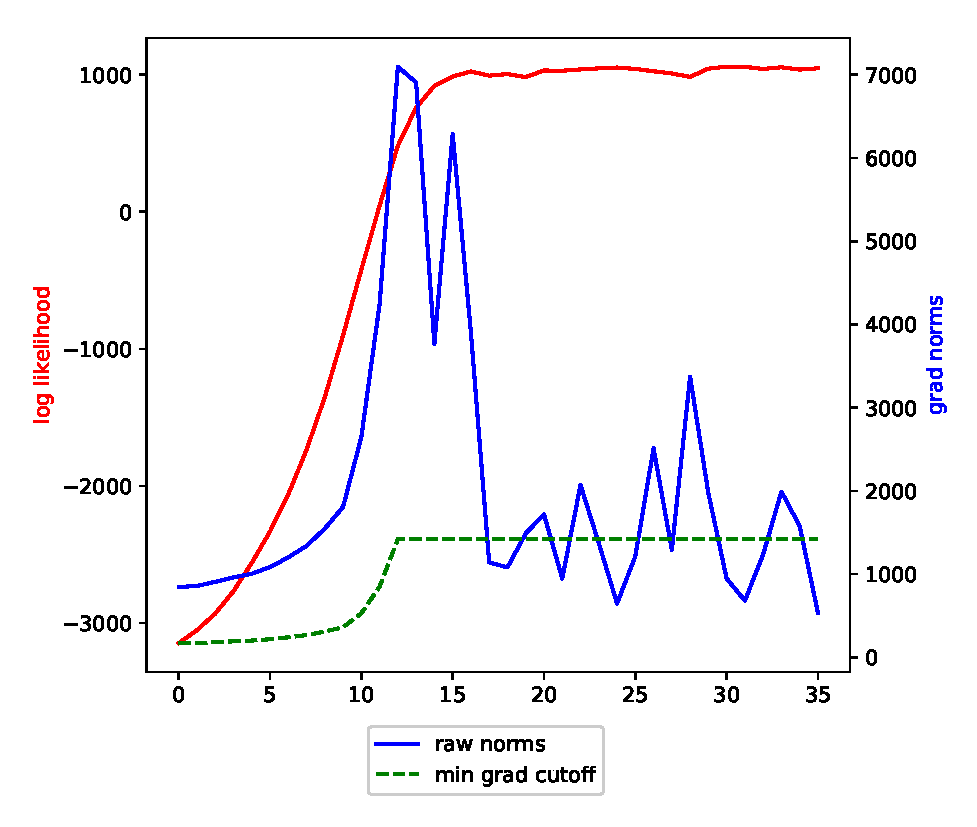
\includegraphics[width=0.5\columnwidth]{running_cutoff.eps}}
\caption{In green, we have 20\% of the rolling maximum norm. In red and blue are $\mcL$ (computed exactly and therefore unavailable during benchmarks) and $ \norm{\nabla\mcL}_\infty $, respectively. }
\label{fx2007-stop}
\end{figure}

\subsection{Prediction}

The predictive mean can be computed in $O(1)$ time as observed in \cite{msgp} by $K_{*,X}\bsa\approx W_{*,\TU}K_{\TU,\TU}\bsa$.

The full predictive covariance estimate requires finding a new term $K_{*,X}K_{X,X}^{-1}K_{X,*}$. This is done by solving the linear system in a matrix-free manner on-the-fly; in particular, $K_{X,X}^{-1}K_{X,*}$ is computed via \textsc{minres} for every new test point $K_{X,*}$. Over several test points, this is embarrassingly parallelizable.

A more efficient predictive variance algorithm is outside the scope of this paper: for a research setting, we expect training time to be the bottleneck. Moreover, one can couple LLGP learning with other prediction mechanisms. One example is the sampling-based approach proposed in \cite{papandreou2011efficient}, which extends to linear combinations of kernels that allow fast eigendecompositions.

\section{Results}
\label{sec:results}
We evaluate the methods on held out data by using standardized mean square error (SMSE) of the test points with the predicted mean, and the negative log predictive density (NLPD) of the Gaussian likelihood of the inferred model. Notably, NLPD takes confidence into account, while SMSE only evaluates the mean prediction. In both cases, lower values represent better performance. We evaluated the performance of our flexible representations of the kernel, \textsc{sum}, \textsc{bt}, and \textsc{slfm}, by computing exact log-likelihood gradients using the standard Cholesky algorithm for a grid of different kernels; this evaluation is available in the paper supplement.\footnote{Hyperparameters for the stopping condition, code, and benchmarking scripts are available in <anonymous repository>.}

\subsection{Foreign exchange rate prediction (FX2007)}\label{fx2007-results}

We replicate the medium-sized dataset from COGP as an application to evaluate LLGP performance. The dataset consists of ten foreign currency exchange rates---CAD, EUR, JPY, GBP, CHF, AUD, HKD, NZD, KRW, and MXN---and three precious metals---XAU, XAG, and XPT---implying that $D=13$.\footnote{Data are from \url{http://fx.sauder.ubc.ca/data.html}} As in COGP, we retrieved the asset to USD rate, then used its reciprocal in all the results discussed below. The LLGP setting has $Q=1,R=2$, as recommended in \cite{alvarez2010efficient} for LMC models on this dataset; let this be the LMC model on LLGP. COGP roughly corresponds to the the SLFM model, which has a total of 94 hyperparameters, compared to 53 for LLGP. All kernels are RBF. The data used in this example are from 2007, and include $n=3054$ training points and $150$ test points. The test points include 50 contiguous points extracted from each of the CAD, JPY, and AUD exchanges. For this application, LLGP uses $m=n/D=238$ interpolating points. We use the COGP settings from the paper.\footnote{COGP hyperparameters for FX2007 were 100 inducing points, 500 iterations, 200 mini-batch size.} LLGP, for both LMC, outperforms COGP in terms of predictive mean and variance estimation as well as runtime (Tab.~\ref{fx2007-tbl}).

\begin{table}[!h]
  \caption{Average predictive performance and training time over $10$ runs for LLGP and COGP on the FX2007 dataset. Parenthesized values are standard error. LLGP was run with LMC set to $Q=1$, $R=2$, and $238$ interpolating points. COGP used a $Q=2$ kernel with $100$ inducing points.}
\label{fx2007-tbl}
\begin{center}
  \begin{small}
    \begin{sc}
      \begin{tabular}{|l|cc|}\hline\abovespace\belowspace
Metric & LLGP & COGP\\
\hline\abovespace
seconds & $100$ ($13$) & \textbf{$731$ ($194$)}\\
SMSE & $0.21$ ($0.01$) & \textbf{$0.26$ ($0.03$)}\\
NLPD & \textbf{$-3.62$ ($0.07$)} & $14.52$ ($3.10$)\\

\belowspace \\
\hline
\end{tabular}

\end{sc}
\end{small}
\end{center}
\end{table}

\begin{figure}[!h]
\centering
{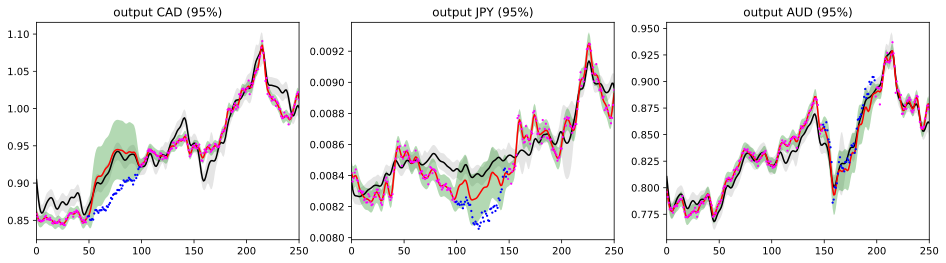
\includegraphics[width=\textwidth]{fx2007graph.pdf}}
\caption{Test outputs for the FX2007 dataset. COGP mean is black, with 95\% confidence intervals shaded in grey. LLGP mean is a solid red curve, with light green 95\% confidence intervals. Magenta points are in the training set, while blue ones are in the test set. Notice LLGP variance corresponds to an appropriate level of uncertainty on the test set and certainty on the training set, as opposed to the uniform variance from COGP.}
\label{fx2007-graph}
\end{figure}

\subsection{Weather dataset}\label{large-bench}

Next, we replicate results from a weather dataset, a large time series used to validate COGP. In this dataset, $D=4$ weather sensors Bramblemet, Sotonmet, Cambermet, and Chimet record air temperature over five days in five minute intervals, with some dropped records due to equipment failure. Parts of Cambernet and Chimet are dropped for imputation, yielding $n=15789$ training measurements and $374$ test measurements. 

We use the COGP parameters that were set by default in the code provided by the authors.\footnote{\url{https://github.com/trungngv/cogp}, commit \texttt{3b07f621ff11838e89700cfb58d26ca39b119a35}. The weather dataset was run on 1500 iterations, mini-batch size 1000.} LLGP was run with the same parameters as in FX2007, simulating the SLFM model. We tested LLGP models on different numbers of interpolating points $m$.

\begin{table}[!h]
  \caption{Average predictive performance and training time over $10$ runs for LLGP and COGP on the weather dataset. Parenthesized values are standard error. Both LLGP and COGP trained the SLFM model. We show LLGP with $500$ and $1000$ interpolating points and COGP with $200$ inducing points.}
\label{weather-tbl}
\begin{center}
  \begin{small}
    \begin{sc}
      \begin{tabular}{|l|ccc|}\hline\abovespace\belowspace
Metric & \begin{tabular}{c}LLGP\\$m=500$\end{tabular} & \begin{tabular}{c}LLGP\\$m=1000$\end{tabular} & COGP\\
\hline\abovespace
seconds & $67$ ($14$) & \textbf{$301$ ($75$)} & $1711$ ($109$)\\
SMSE & $0.09$ ($0.01$) & $0.09$ ($0.01$) & $0.08$ ($0.00$)\\
NLPD & $2.14$ ($0.58$) & $1.54$ ($0.03$) & $98.48$ ($1.30$)
\belowspace \\
\hline
\end{tabular}

\end{sc}
\end{small}
\end{center}
\end{table}

LLGP performed slightly worse than COGP in SMSE, but both NLPD and runtime indicate significant improvements (Tab.~\ref{weather-tbl}). Varying the number of interpolating points $m$ from $500$ to $1000$ constructs a tradeoff frontier between increases in $m$ and NLPD decrease at the cost of additional runtime (Fig.~\ref{fig:llgpweather}). While NLPD improvement diminishes as $m$ increases, LLGP is still an improvement compared to COGP for a range of $m$ by an order of magnitude in runtime and almost two orders of magnitude for NLPD.

\begin{figure}[!h]
\centering
{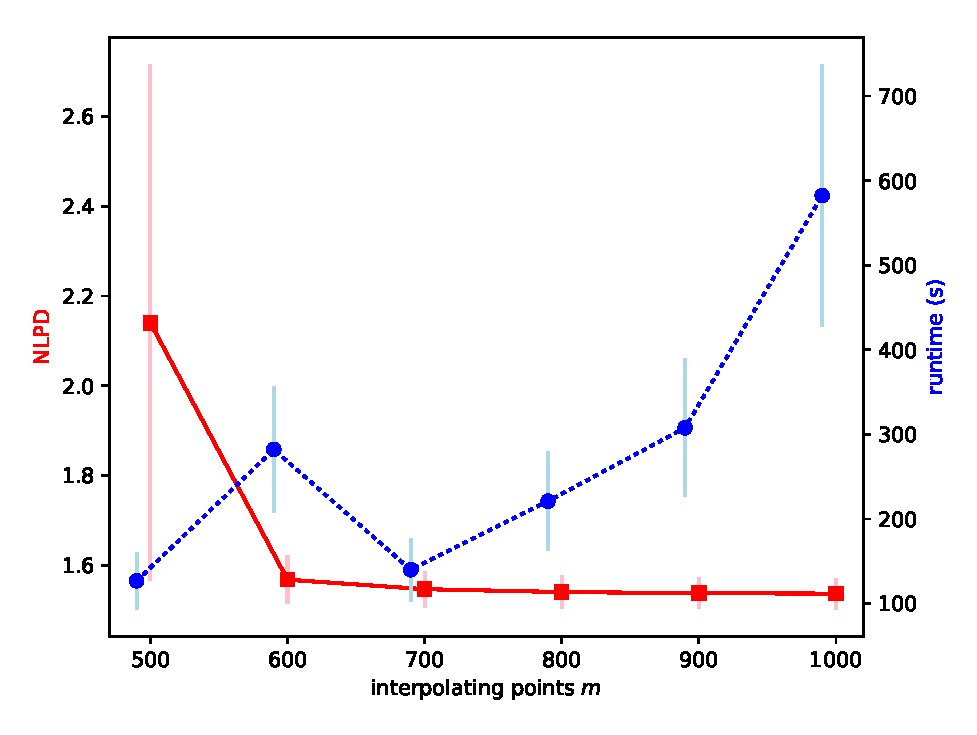
\includegraphics[width=0.5\columnwidth]{m_time_nlpd.eps}}
\caption{Average and standard error of NLPD and runtime of the SLFM model on LLGP across over varying interpolating points. Every setting was run 10 times.}
\label{fig:llgpweather}
\end{figure}
\section{Conclusion}\label{conclusion}

LLGP recovers speedups from SKI \cite{kiss-gp} for the problem of multi-output GP regression by recognizing structure unique to LMC kernels, and otherwise not necessarily recoverable in general multi-output kernels. This structure further enables a parsimonious representation that allows even large GPs to be learned without explicit construction of the covariance matrix.

LLGP provides a means to approximate the log-likelihood function gradients through interpolation. We have shown on several datasets that this can be done in a way that is faster and leads to more accurate results than variational approximations. Because LLGP's representation can be efficient without being sparse (i.e., $m$ may be large), it can can capture complex interactions in the covariance. As pictured in Fig.~\ref{fx2007-graph}, and demonstrated by NLPD performance on both the FX2007 and weather datasets (Tab.~\ref{fx2007-tbl},\ref{weather-tbl}), such an efficient, non-sparse representation is integral to making a model whose confidence at a test site reflects the amount of related training data for that site.

Future work would extend the inputs to accept multiple dimensions. This can be done without losing internal structure in the kernel \cite{msgp}: Toeplitz covariance matrices become block-Toeplitz with Toeplitz-blocks (BTTB). The cubic interpolation requires and exponential number of terms, so projection into lower dimensions learned in a supervised manner would be essential. Another useful line for investigation would be more informed stopping heuristics. Finally, an extension to non-Gaussian noise is also feasible in a matrix-free manner by following prior work \cite{cutajar2016preconditioning}.

\bibliographystyle{unsrtnat}
\bibliography{paper}


\end{document}
